%Ahim� sull?internal note sono stati di poche parole sulla parte di mono-jet per 2HDM+a.
%Comunque gran parte dei risultati che ho prodotto sono sintetizzati in https://indico.cern.ch/event/660808/contributions/2697161/attachments/1510819/2355991/2017.08.21.2HDMaMonojet.pdf.

\subsubsection{Monojet}

The search for events with at least one jet and large missing transverse momentum in the final states can be also interpreted in the context of the 2HDM+a model. In this scenario the light pseudo-scalar mediator which decays in DM particles can be radiated from heavy quark loops providing such a signature. This channel is able to probe a phase space with low $\tan(\beta)$ and high $\sin\theta$ in which the cross-sections of this kind of processes are enhanced.

\subsubsection{Resonant Production at Collider (Comparison)}

\begin{figure}
\begin{center}
%\vspace*{1.5cm} 
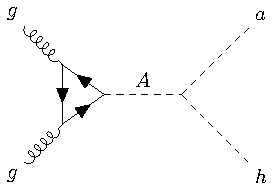
\includegraphics[width=0.4\textwidth]{texinputs/04_grid/figures/MonoHiggsAa.pdf}
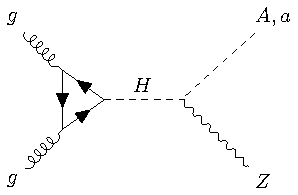
\includegraphics[width=0.4\textwidth]{texinputs/04_grid/figures/MonoZHAa.pdf} \vspace{2em}\\
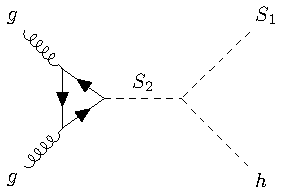
\includegraphics[width=0.4\textwidth]{texinputs/04_grid/figures/MonoHiggsS2S1.pdf}
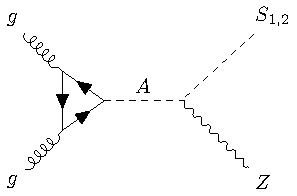
\includegraphics[width=0.4\textwidth]{texinputs/04_grid/figures/MonoZAS12.pdf}
\caption{Feynman diagrams for resonant production signals signatures leading to mono-Z or mono-h.} 
\label{fig:feynresprod}
\end{center}
\end{figure}

The cross section for a resonant production process, with final state X, where a spin-0 resonance $S$ is produced and then decays, can be written as

\begin{eqnarray}
\sigma(p p \rightarrow S \rightarrow X) &=& \frac{\Gamma(S\rightarrow X)}{M \Gamma s} \sum_{i} C_{i} \Gamma(S\rightarrow i) = \frac{1}{M  s} \sum_{i} C_{i} \Gamma(S\rightarrow i) BR(S\rightarrow X)
\end{eqnarray}

where $i$ are the possible initial states, $C_i$ are weight factors that account for the protons PDFs and colour factors, and $s$ is the center of mass energy squared $s=(13TeV)^2$.

The values of the $C_i$ are as follows

\begin{eqnarray}
C_{gg} &=& \frac{\pi^2}{8} \int_{M^2/s}^1 \frac{dx}{x} g(x)g\left(\frac{M^2}{sx}\right)\\
C_{q\bar{q}} &=& \frac{4\pi^2}{9} \int_{M^2/s}^1 \frac{dx}{x}\left(q(x)\bar{q}\left(\frac{M^2}{sx}\right) + q\left(\frac{M^2}{sx}\right)\bar{q}(x)\right)
\end{eqnarray}

Assuming gluon fusion production to be the dominant one, the ratio of the cross sections for the scalar and pseudoscalar model for mono-higgs and mono-Z will be

\begin{eqnarray}
\frac{\sigma_S(p p \rightarrow S_2 \rightarrow \bar{\chi}\chi h)}{\sigma_P(p p \rightarrow A \rightarrow \bar{\chi}\chi h)} &=& \frac{\Gamma(S_2\rightarrow gg)}{\Gamma(A\rightarrow gg)} \frac{BR(S_2\rightarrow S_1 h)}{BR(A\rightarrow a h)} \frac{BR(S_1\rightarrow \bar{\chi}\chi)}{BR(a\rightarrow \bar{\chi}\chi)}\\
\frac{\sigma_S(p p \rightarrow A \rightarrow \bar{\chi}\chi Z)}{\sigma_P(p p \rightarrow H \rightarrow \bar{\chi}\chi Z)} &=& \frac{\Gamma(A\rightarrow gg)}{\Gamma(H\rightarrow gg)} \frac{BR(A\rightarrow S_1 Z)}{BR(H\rightarrow a Z)} \frac{BR(S_1\rightarrow \bar{\chi}\chi)}{BR(a\rightarrow \bar{\chi}\chi)}
\end{eqnarray}

The ideal situation to detect a mono-higgs/Z signal is to have such BR close to 1: if this is the case, the ratio of the signals becomes just the ratio of the widths

\begin{eqnarray}
\frac{\sigma_S(p p \rightarrow S_2 \rightarrow \bar{\chi}\chi h)}{\sigma_P(p p \rightarrow A \rightarrow \bar{\chi}\chi h)} &\sim& \frac{\Gamma(S_2\rightarrow gg)}{\Gamma(A\rightarrow gg)} \label{eq:sigmamonohapprox}\\
\frac{\sigma_S(p p \rightarrow A \rightarrow \bar{\chi}\chi Z)}{\sigma_P(p p \rightarrow H \rightarrow \bar{\chi}\chi Z)} &\sim& \frac{\Gamma(A\rightarrow gg)}{\Gamma(H\rightarrow gg)} \label{eq:sigmamonozapprox}
\end{eqnarray}

\begin{figure}
\begin{center}
%\vspace*{1.5cm} 
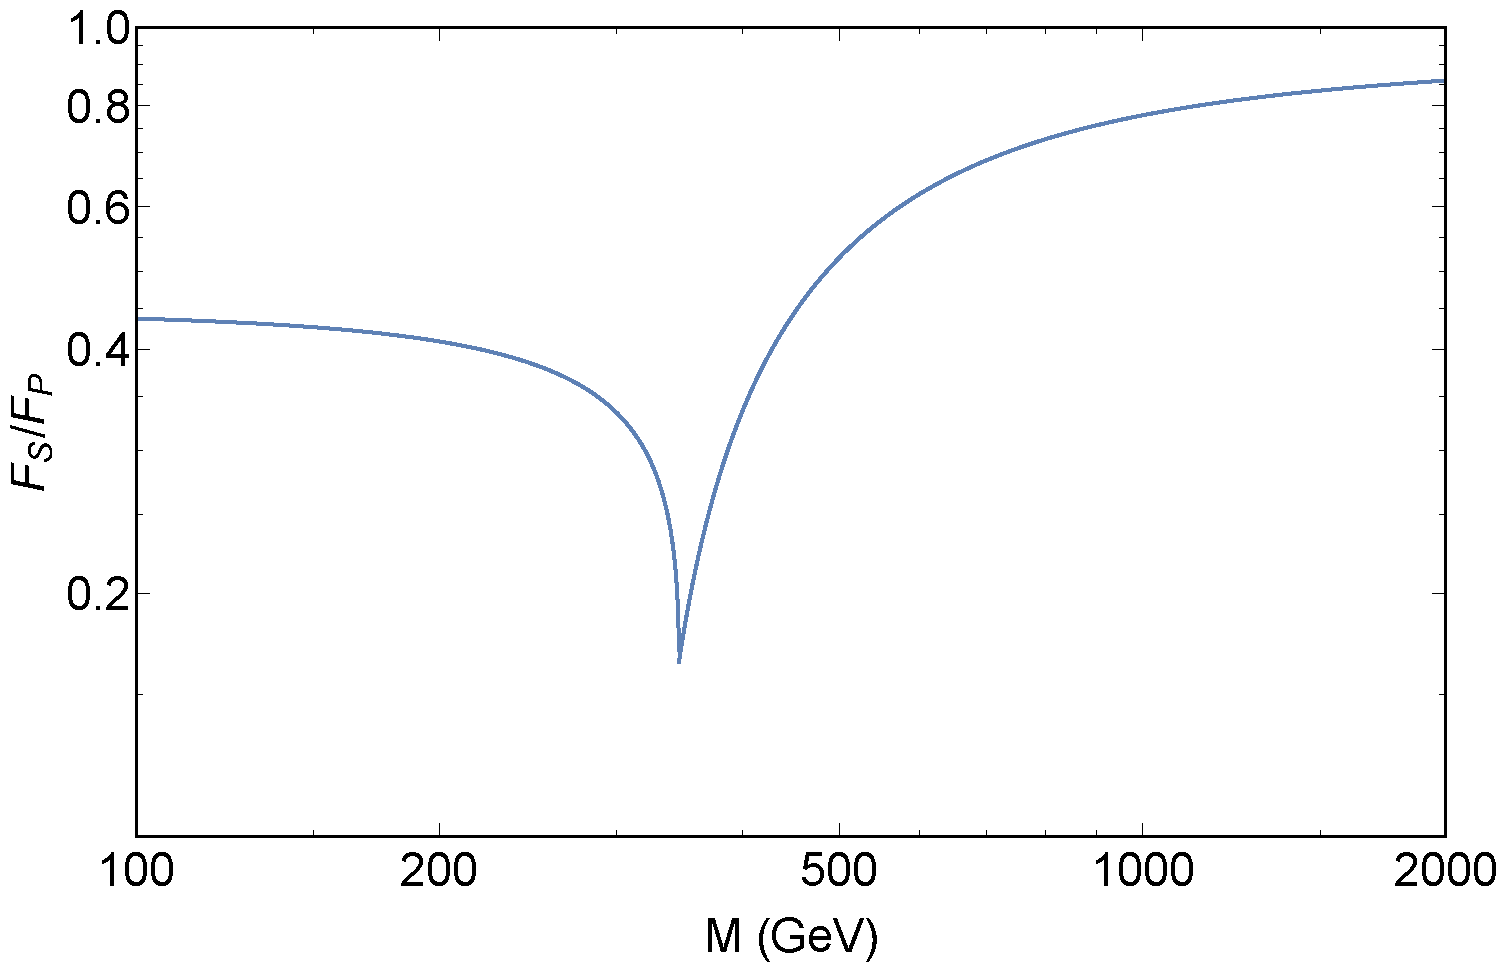
\includegraphics[width=0.7\textwidth]{texinputs/04_grid/figures/ratio.pdf}
\caption{Ratio $F_S/F_P$ as a function of the mass $M=M_A=M_{S_2}$.} 
\label{fig:resonantratio}
\end{center}
\end{figure}

the width for a scalar or pseudoscalar particle to gluons are:

\begin{eqnarray}
\Gamma(S\rightarrow gg) &=& \frac{g_S^2 \alpha_s^2 M}{16\pi^3} F_S\left(\frac{4m_t^2}{M^2}\right)\\
\Gamma(P\rightarrow gg) &=& \frac{g_P^2 \alpha_s^2 M}{16\pi^3} F_P\left(\frac{4m_t^2}{M^2}\right)
\end{eqnarray}
where
\begin{eqnarray}
F_S(x) &=& x |1+(1-x)\arctan^2\frac{1}{\sqrt{x-1}} |^2\\
F_P(x) &=& x |\arctan^2\frac{1}{\sqrt{x-1}} |^2
\end{eqnarray}

and $g_S = -y_t \sin\theta \epsilon_u$ for $S=S_2$, $g_P = y_t \epsilon_u$ for $A$ in the scalar model, and $g_S= y_t \epsilon_u$ for $S=H$, $g_P = y_t \cos\theta \epsilon_u$ for $A$ in the PS model. Note that the definition of the mixing angle is reversed in the scalar model comparing to the PS. So assuming equivalent mixing angle configurations, Eq. \ref{eq:sigmamonohapprox} and \ref{eq:sigmamonozapprox} reduce to

\begin{eqnarray}
\frac{\sigma_S(p p \rightarrow S_2 \rightarrow \bar{\chi}\chi h)}{\sigma_P(p p \rightarrow A \rightarrow \bar{\chi}\chi h)} &\sim& \frac{F_S(\frac{4m_t^2}{M^2})}{F_P(\frac{4m_t^2}{M^2})} <1 \\
\frac{\sigma_S(p p \rightarrow A \rightarrow \bar{\chi}\chi Z)}{\sigma_P(p p \rightarrow H \rightarrow \bar{\chi}\chi Z)} &\sim& \frac{F_P(\frac{4m_t^2}{M^2})}{F_S(\frac{4m_t^2}{M^2})} >1
\end{eqnarray}

The ratio $F_S/F_P$ is shown in Fig. \ref{fig:resonantratio} as a function of the mass $M=M_A=M_{S_2}$.